\section{Verbesserungsmöglichkeiten}
\color{blue}
Während den Tests, aber auch schon beim Zusammenbau, wurden einige Schwachstellen gefunden, welche aus Zeitgründen oder fehlendem mechanischem Verständnis, welches den Rahmen der Arbeit sprengen würde, nicht verbessert wurden. Auf diese Punkte soll in diesem Kapitel eingegangen werden. Dies aus dem Grund, um solche Fehler bei einem zukünftigen Umbau von Anfang an zu vermeiden oder sie auch im Anschluss an dieses Projekt noch zu verbessern. 

\subsection{Batteriekisten}
Die beiden Kisten für die Batterien sind sehr gross und entsprechend auch schwer. Ausserdem konnten sie nur mit Anpassungen beide im Heck des Fahrzeugs platziert werden, sodass dort der Platz für die Anschlüsse sehr knapp ist. Um eine möglichst hohe Batteriekapazität zu ermöglichen, wurden jeweils drei Zellen parallel geschaltet, worin der Grund für die grossen Batteriekisten zu finden ist. Ausserdem befinden sich in den Batteriekisten jeweils noch die Dioden, die Sicherungen sowie die Batteriemanagementsysteme.

Eine Batteriekiste, welche auf Parallelschaltungen verzichten würde, könnte beide Batterien sowie das wichtige Zubehör (siehe oben) beinhalten und wäre immer noch kleiner als eine einzelne aktuelle Batteriekiste. Als Nachteil dieser Variaton kann die reduzierte Reichweite genannt werden. Aufgrund der geringeren Batteriekapazität beträgt diese nur noch gut ein Drittel (das Fahrzeuggewicht wird ebenfalls merklich reduziert).

Ein weiterer Punkt, welcher bei einer neuen Batterie unbedingt beachtet werden sollte, ist die Zugänglichkeit zu Verschleissteilen, insbesondere den Sicherungen. Der schlechteste Fall, welcher aktuell eintreten kann, ist das Auslösen der Sicherung von Batterie eins. Um diese zu ersetzen muss Batterie zwei (welche auf Batterie eins liegt) entfernt werden und erst anschliessend kann der Deckel von Batterie eins geöffnet werden, womit die Sicherung ersetzt werden kann. Eine neue Batteriekiste sollte unbedingt einen direkten Zugang (beispielsweise eine Seitenöffnung) zur Sicherung ermöglichen.

\subsection{Steuerplatine}
Wie bereits unter \ref{steuerplatine} beschrieben wurde, besitzt die Steuerplatine einen Fehler. Dieser Fehler konnte mit einer Schaltung auf einer zusätzlichen Leiterplatte behoben werden. Diese Lösung ist aber nicht optimal. Eine schöne Lösung wäre eine neue Steuerplatine, welche entweder bereits diese Inverterschaltung oder aber eine komplett andere Schaltung zur Ansteuerung der Komponenten beinhaltet.

\subsection{Tachometer}
Im Fahrzeug ist ein alter Tachometer verbaut, welcher nicht nur die aktuelle Geschwindigkeit in Meilen pro Stunde anzeigen kann, sondern auch die Tagesstrecke sowie die Gesamtstrecke misst. Leider funktioniert dieser Tachometer nicht, da das Zahnrad, welches die Drehung des Rades abgreift, nicht mit dem Rad in Eingriff ist. Dies ist in Abbildung \ref{fig:Zahnrad} gezeigt:

\begin{figure}[h]
	\centering
		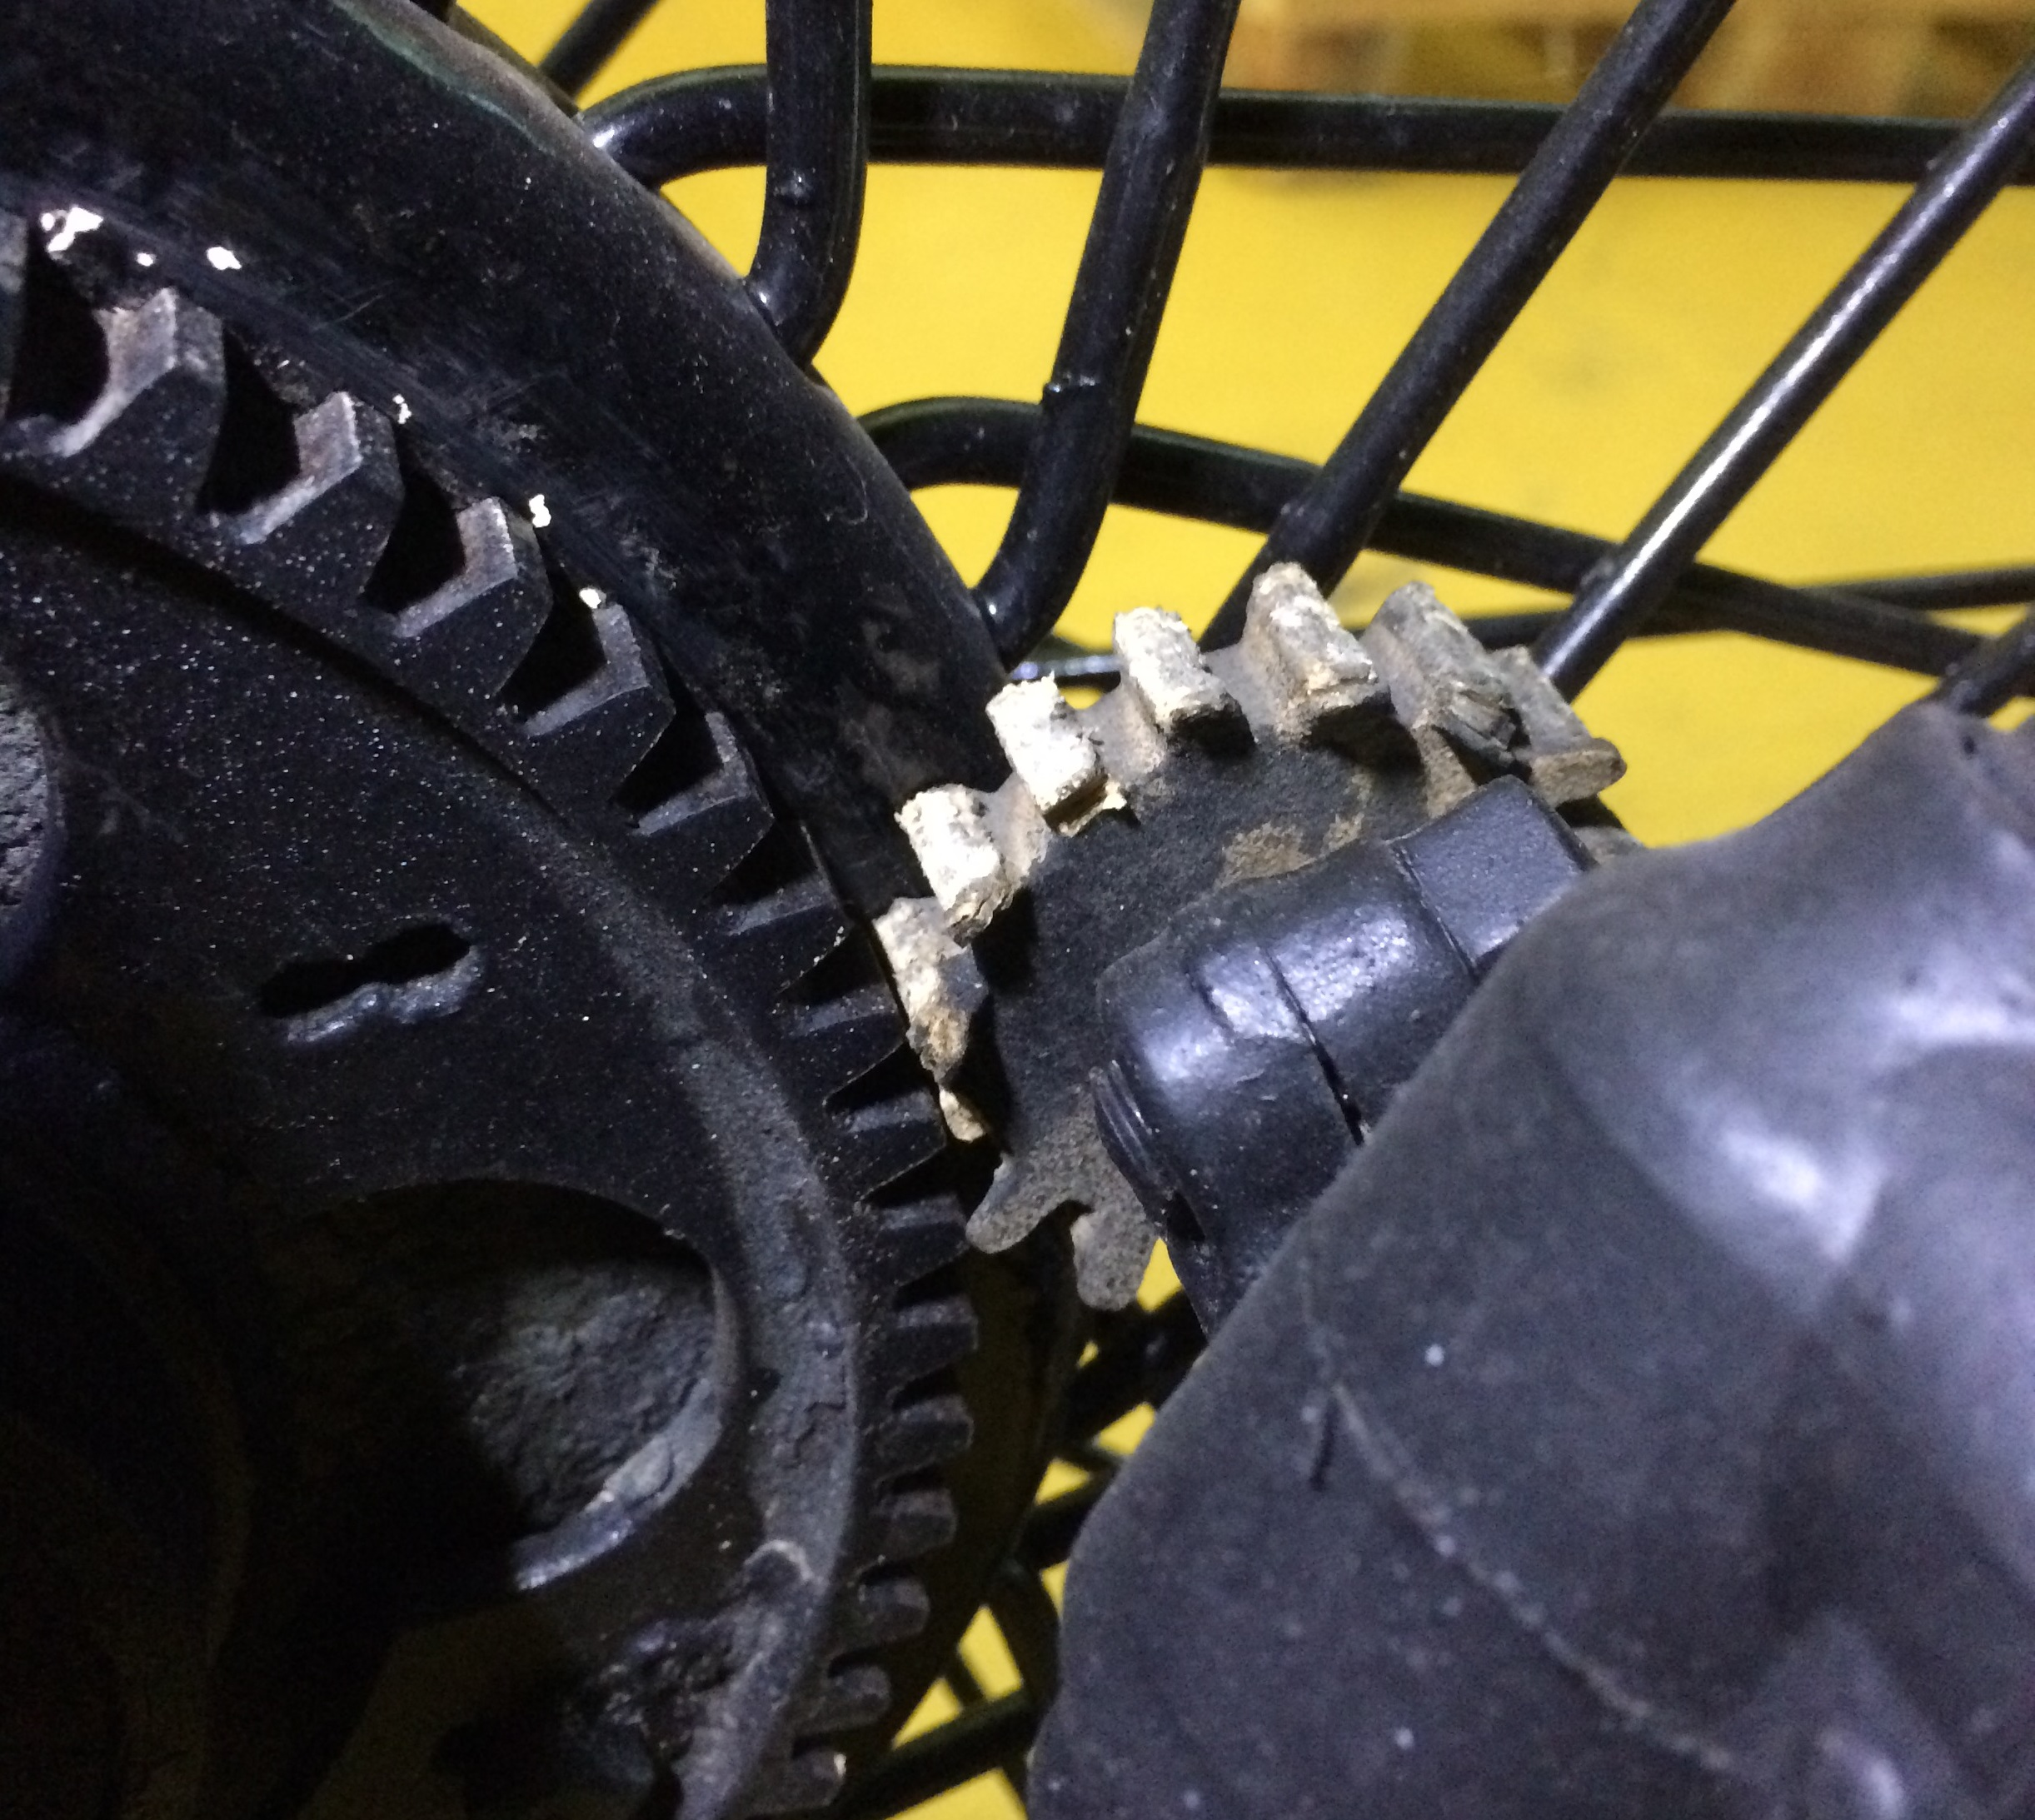
\includegraphics[width=0.70\textwidth]{images/Zahnrad.jpg}
	\caption{Das abgenützte Zahnrad verhindert die korrekte Funktion des Tachometers}
	\label{fig:Zahnrad}
\end{figure}

Der Tachometer selbst wurde ebenfalls getestet. Dieser funktioniert korrekt. Nicht getestet wurde die Sehne als Verbindungselement zwischen Zahnrad und Tachometer, welche ein heikles Bauteil darstellt.

Ein weiteres Problem mit dem Tachometer stellt der Metallschlauch dar, in welchem die Sehne geführt ist. Dieser Schlauch wird an der Stelle durch den Fahrzeugboden geführt, an welcher sich auch der Anfahrwiderstand befindet. Beim Einbau des Bodens muss darauf geachtet werden, dass der Anfahrwiderstand nicht durch den Metallschlauch überbrückt wird, wobei dieser Fall durch einen isolierenden Schrumpfschlach ansatzweise gelöst ist (dies ist jedoch keine dauerhafte Lösung). Auf jeden Fall ist dieser Schlauch aber der Hitze des Anfahrwiderstandes ausgesetzt, weswegen die Positionierung alles andere als ideal ist.

\subsection{Lager}
Die Lager der Hinterräder werden im Betrieb warm, die Temperaturen liegen ungefähr $20^\circ$C über der Umgebungstemperatur. Dieses Problem konnte auch durch ein Nachfüllen des Schmieröles nicht gelöst werden, weswegen hier eine mechanische Kontrolle der Lager nötig ist. Diese wurde nicht durchgeführt, da dafür ein Experte für mechanische Systeme zu Rate gezogen werden muss.

\subsection{Türen}
Die Türen der Fahrerkabinen sind sehr schwer und auch nur mit extremem Schwung zu schliessen. In diesem Fall sollte sich die Türen ebenfalls ein Fachmann anschauen um eventuelle Unebenheiten oder Verbiegungen im Gehäuse der Türen zu verbessern, damit man diese normal zu bringt.

\subsection{Stufenschalter}
Im offenen Zustand (ohne Kabinenboden und Stufenschalterdeckel) funktioniert der Stufenschalter problemlos. Im zusammengebauten Zustand konnte allerdings ein Problem beim Einlegen der Rückwärtsstufen beobachtet werden: Der erste Gang rückwärts, welcher für Manöver benötigt wird, lässt sich nicht immer problemlos einlegen. Manchmal springt der Stufenschalter direkt zu Stufe zwei, überbrückt also den Anfahrwiderstand. Es wird stark vermutet, dass es ein mechanisches Problem ist, bei welchem beispielsweise irgendwo eine Stange einen erhöhten Widerstand hat. Da die mechanische Steuerung aber sehr aufwändig ist konnte die Problemstelle bei Tests im Stillstand nicht geortet werden.

\subsection{Volt- und Amperemeter}

\color{black}